\clearpage\begingroup\SourceLeaf{116b}\HistoricalHead{111}{R}{GAUSS AN GERLING UND OLBERS.}
\newcommand{\HistoricalCurrencyTwentyThreeA}{%
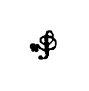
\begin{tikzpicture}[x=0.1666667pt,y=-0.1666667pt,baseline=-11pt]
\path[use as bounding box] (0,0) rectangle (71,77);
\path[fill=black,even odd rule] (51,6) -- (44,6) -- (43,7) -- (42,7) -- (40,9) -- (40,11) -- (39,12) -- (39,14) -- (36,17) -- (35,17) -- (34,18) -- (32,18) -- (29,21) -- (28,21) -- (26,23) -- (26,31) -- (29,34) -- (30,34) -- (32,36) -- (33,36) -- (36,38) -- (36,40) -- (37,41) -- (37,45) -- (36,46) -- (30,44) -- (26,40) -- (26,39) -- (22,35) -- (20,35) -- (17,37) -- (14,34) -- (9,34) -- (8,35) -- (7,35) -- (5,38) -- (5,44) -- (8,47) -- (8,50) -- (10,52) -- (13,52) -- (14,51) -- (15,51) -- (18,53) -- (20,53) -- (24,49) -- (24,48) -- (22,46) -- (23,45) -- (24,45) -- (26,47) -- (29,47) -- (34,51) -- (36,51) -- (37,52) -- (37,53) -- (38,54) -- (38,56) -- (39,57) -- (39,60) -- (35,65) -- (34,65) -- (31,62) -- (31,61) -- (30,60) -- (26,60) -- (23,63) -- (23,67) -- (26,69) -- (32,69) -- (33,68) -- (40,68) -- (41,67) -- (42,67) -- (44,65) -- (44,63) -- (46,60) -- (46,51) -- (49,48) -- (56,48) -- (57,47) -- (58,47) -- (58,46) -- (61,43) -- (61,41) -- (62,40) -- (62,38) -- (63,37) -- (63,31) -- (62,30) -- (62,27) -- (56,21) -- (56,17) -- (57,16) -- (56,15) -- (56,14) -- (55,13) -- (55,12) -- (54,11) -- (53,8) -- cycle
(57,28) -- (59,31) -- (59,39) -- (57,41) -- (54,42) -- (52,44) -- (50,44) -- (49,45) -- (47,45) -- (45,43) -- (47,37) -- (48,36) -- (49,36) -- (49,35) -- (50,34) -- (51,34) -- (52,33) -- (52,32) -- (56,28) -- cycle
(46,22) -- (47,23) -- (51,23) -- (53,25) -- (53,27) -- (47,33) -- (45,31) -- (45,30) -- (44,29) -- (45,28) -- (45,23) -- cycle
(34,22) -- (35,22) -- (36,23) -- (36,28) -- (37,29) -- (37,31) -- (35,33) -- (34,33) -- (30,29) -- (30,25) -- (32,23) -- (33,23) -- cycle
(44,13) -- (47,10) -- (48,10) -- (52,14) -- (53,17) -- (52,18) -- (50,18) -- (49,17) -- (46,17) -- (44,15) -- cycle;
\end{tikzpicture}}
\newcommand{\HistoricalCurrencyTwentyThreeB}{%
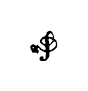
\begin{tikzpicture}[x=0.1666667pt,y=-0.1666667pt,baseline=-11pt]
\path[use as bounding box] (0,0) rectangle (70,76);
\path[fill=black,even odd rule] (50,7) -- (46,7) -- (45,8) -- (44,8) -- (41,11) -- (41,13) -- (40,14) -- (40,16) -- (37,19) -- (36,19) -- (35,20) -- (33,20) -- (28,25) -- (28,26) -- (27,27) -- (27,32) -- (31,36) -- (32,36) -- (34,38) -- (35,38) -- (38,41) -- (38,42) -- (39,43) -- (39,47) -- (38,48) -- (33,48) -- (31,46) -- (30,46) -- (21,37) -- (19,39) -- (17,39) -- (15,37) -- (14,37) -- (13,36) -- (10,36) -- (6,40) -- (6,45) -- (7,46) -- (7,48) -- (9,50) -- (9,53) -- (10,53) -- (11,54) -- (19,54) -- (21,56) -- (22,56) -- (24,53) -- (24,50) -- (22,48) -- (21,45) -- (22,44) -- (24,44) -- (26,46) -- (26,47) -- (27,48) -- (30,49) -- (32,51) -- (34,51) -- (36,53) -- (38,53) -- (40,55) -- (40,58) -- (39,59) -- (39,66) -- (36,69) -- (34,67) -- (34,63) -- (33,62) -- (29,62) -- (26,65) -- (26,70) -- (29,72) -- (38,72) -- (39,71) -- (40,71) -- (43,68) -- (43,67) -- (46,64) -- (46,63) -- (47,62) -- (47,54) -- (49,52) -- (50,52) -- (51,51) -- (53,51) -- (55,49) -- (57,49) -- (63,43) -- (63,42) -- (64,41) -- (64,33) -- (63,32) -- (63,30) -- (62,29) -- (62,28) -- (57,23) -- (57,19) -- (56,18) -- (56,15) -- (54,13) -- (54,11) -- cycle
(10,43) -- (11,42) -- (13,42) -- (14,43) -- (14,44) -- (13,45) -- (11,45) -- (10,44) -- cycle
(59,30) -- (61,32) -- (61,39) -- (60,40) -- (60,41) -- (56,45) -- (55,45) -- (52,48) -- (49,49) -- (46,46) -- (47,45) -- (47,39) -- (48,38) -- (50,38) -- (50,37) -- (55,32) -- (55,31) -- (56,30) -- cycle
(33,25) -- (37,25) -- (38,26) -- (38,31) -- (39,32) -- (39,34) -- (38,35) -- (35,35) -- (34,34) -- (33,34) -- (32,33) -- (32,31) -- (31,31) -- (30,30) -- (30,29) -- (32,27) -- (32,26) -- cycle
(47,23) -- (48,23) -- (49,24) -- (52,25) -- (54,27) -- (54,29) -- (51,32) -- (51,33) -- (49,35) -- (47,35) -- (46,34) -- (46,29) -- (45,28) -- (45,26) -- cycle
(45,16) -- (49,12) -- (50,12) -- (54,16) -- (54,18) -- (55,19) -- (55,20) -- (54,21) -- (51,21) -- (50,20) -- (46,20) -- (45,19) -- cycle;
\end{tikzpicture}}
\newcommand{\HistoricalCurrencyTwentySix}{%
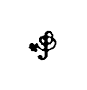
\begin{tikzpicture}[x=0.1250000pt,y=-0.1250000pt,baseline=-11pt]
\path[use as bounding box] (0,0) rectangle (90,99);
\path[fill=black,even odd rule] (67,10) -- (64,10) -- (63,9) -- (56,9) -- (55,10) -- (55,11) -- (54,12) -- (52,12) -- (51,13) -- (51,15) -- (50,16) -- (49,16) -- (49,21) -- (47,23) -- (44,23) -- (42,25) -- (39,25) -- (38,26) -- (36,26) -- (35,29) -- (33,31) -- (33,40) -- (39,46) -- (39,48) -- (41,50) -- (44,50) -- (48,55) -- (48,59) -- (45,62) -- (42,62) -- (41,61) -- (40,61) -- (31,52) -- (31,51) -- (30,50) -- (30,48) -- (27,45) -- (25,45) -- (21,49) -- (19,49) -- (15,45) -- (9,45) -- (5,49) -- (5,55) -- (3,57) -- (3,58) -- (5,60) -- (7,60) -- (9,62) -- (9,65) -- (12,68) -- (19,68) -- (21,70) -- (25,70) -- (28,67) -- (28,64) -- (27,63) -- (27,62) -- (26,62) -- (25,61) -- (25,60) -- (28,57) -- (31,60) -- (33,60) -- (34,61) -- (35,61) -- (38,64) -- (40,64) -- (42,66) -- (42,67) -- (45,67) -- (46,68) -- (48,68) -- (49,69) -- (49,83) -- (48,84) -- (48,85) -- (45,88) -- (44,88) -- (41,85) -- (43,83) -- (38,79) -- (34,79) -- (32,81) -- (29,82) -- (29,85) -- (31,87) -- (31,89) -- (33,91) -- (36,91) -- (39,94) -- (43,94) -- (44,93) -- (48,93) -- (50,91) -- (51,91) -- (55,87) -- (55,86) -- (58,83) -- (58,70) -- (63,65) -- (64,65) -- (65,64) -- (67,64) -- (68,63) -- (71,63) -- (73,61) -- (74,61) -- (80,55) -- (80,52) -- (81,51) -- (81,50) -- (83,48) -- (83,39) -- (81,37) -- (81,36) -- (73,28) -- (73,26) -- (74,25) -- (74,20) -- (71,17) -- (71,16) -- (70,15) -- (70,13) -- (69,12) -- (68,12) -- (67,11) -- cycle
(75,39) -- (78,42) -- (78,47) -- (77,48) -- (77,50) -- (75,52) -- (75,54) -- (71,58) -- (68,58) -- (65,61) -- (62,61) -- (61,62) -- (59,62) -- (57,60) -- (57,58) -- (58,57) -- (58,51) -- (61,48) -- (66,48) -- (67,47) -- (67,46) -- (69,44) -- (70,44) -- (70,42) -- (73,39) -- cycle
(42,32) -- (44,32) -- (45,33) -- (45,34) -- (48,36) -- (48,42) -- (45,45) -- (41,41) -- (41,39) -- (40,38) -- (40,35) -- cycle
(61,29) -- (65,29) -- (68,32) -- (68,36) -- (67,37) -- (67,39) -- (63,43) -- (61,43) -- (58,40) -- (58,32) -- (59,31) -- (60,31) -- (60,30) -- cycle
(61,15) -- (64,15) -- (68,19) -- (68,21) -- (69,22) -- (69,24) -- (67,26) -- (65,26) -- (64,25) -- (61,25) -- (60,24) -- (60,23) -- (58,23) -- (57,22) -- (57,19) -- cycle;
\end{tikzpicture}}

\begin{center}[26.]\end{center}
\begin{center}\textsc{Gauss} an \textsc{Olbers}.\quad Göttingen, 2. September 1837.\end{center}
\begin{center}\begin{minipage}{.88\linewidth}\centering\hrule\vspace{3pt}
\small [\textsc{Wilhelm Olbers}, Sein Leben und seine Werke II, 2, S. 649.]
\par\vspace{3pt}\hrule\end{minipage}\end{center}
\noindent .\ .\ .\ .\ .\ .\ .\ .\ .\ .\ .\ .\ .\ .\ .\ .\ .\ .\ .\ .\ .\par
\indent In der Sitzung der Societät im Jubiläum (19. September) werde ich eine
Vorlesung halten über ein neues Mittel für die Magnetischen Beobachtungen\textsuperscript{[*)]}.
Es bezieht sich auf einen neuen Apparat, der für die (horizontale) Intensität
\begingroup\renewcommand{\thefootnote}{}\footnotetext{[*) Siehe den Bericht über die am 19. September 1837 gehaltene Vorlesung: \textit{Ein neues Hülfsmittel für die Magnetischen Beobachtungen} in den Göttingischen Gelehrten Anzeigen vom 30. Oktober 1837, Werke V, S. 352, und den Aufsatz \textit{Über ein neues, zunächst zur unmittelbaren Beobachtung der Veränderungen in der Intensität des horizontalen Theils des Erdmagnetismus bestimmtes Instrument} in den Resultaten aus den Beobachtungen des magnetischen Vereins im Jahre 1837, S. 1, Werke V, S. 357.]}\endgroup
\clearpage\SourceLeaf{117}\HistoricalHead{112}{L}{PHYSIK. BRIEFWECHSEL.}
\noindent ganz dasselbe leistet, was das Magnetometer für die Declination, wodurch
also die Aufgabe (Resultate, S. 12\textsuperscript{[*)]}), soweit von dem horizontalen Theile der
Erdmagnetischen Kraft die Rede ist, erledigt wird. Von einer rohen Probe
der Grundidee finden Sie eine Andeutung in \textsc{Schumachers} Jahrbuch 1836,
S. 19\textsuperscript{[**)]}, woraus freilich nicht zu erkennen ist, \textls[120]{in was} das Mittel besteht,
sondern nur ein secundärer Theil von dem, was \textls[120]{damit} geschieht. In diesem
Sommer habe ich aber den Apparat ordentlich ausführen lassen, und es sind
sogar die beiden letzten Termine (der Haupttermin vom 29. Juli und der
Extratermin vom 31. August) vollständig damit beobachtet, während ebenso
vollständig in beiden auch im M[agnetischen] O[bservatorium] der Verlauf
der Declination beobachtet ist.
\begingroup\renewcommand{\thefootnote}{}\footnotetext{[*) \textit{Einleitung}, Resultate aus den Beobachtungen des magnetischen Vereins im Jahre 1836, S. 1, Werke V, S. 345, siehe insbesondere S. 351.]}
\footnotetext{[**) \textit{Erdmagnetismus und Magnetometer}, Werke V, S. 315, siehe insbesondere S. 326 Zeile 4 v. u. bis S. 327 Zeile 2.]}\endgroup

Der horizontale Theil des Erdmagnetismus kann also jetzt so scharf beobachtet
werden, wie die Sterne am Himmel. Aber mit dem verticalen
Theile wird eine ähnliche Genauigkeit \textls[120]{niemals} erreicht werden können;
wer die Stelle der \textit{Intensitas vis etc.} p. 15 »Ex hoc rem — requiratur«\textsuperscript{[***)]} gehörig
studirt und beherzigt hat, wird diess leicht von selbst einsehen. Wenn
man aber auch nicht die gleiche Genauigkeit wie bei dem horizontalen Theil
erreichen kann, so bin ich doch überzeugt, dass man viel mehr erreichen
kann, als bis jetzt erreicht ist. Das ist aber etwas, worauf ich mich nicht
einlassen kann. Bei den Instrumental-Hülfsmitteln für die beiden Elemente
des horizontalen Theils konnten geistige Mittel ausreichen, d. i. durch eine
\textls[120]{gehörige Einrichtung} konnte man Apparate zur Erreichung der höchsten
Genauigkeit darstellen, die eigentlich keine übermässig feine mechanische Arbeit
erfordern, und mit geringen Kosten angefertigt werden können. (Der
neue Apparat kommt nicht auf 50 \HistoricalCurrencyTwentySix, natürlich alles schon vorhandene, was
dabei gebraucht wird, ungerechnet, namentlich Uhr, Theodolith und Magnetstab.)
Dagegen sind bei allem, wobei der verticale Theil der magnetischen
Kraft auf irgend eine Art mit ins Spiel kommt, sei es als Inclination oder
anders, sehr fein, sehr vollkommen ausgearbeitete, also auch am Ende kost-
\begingroup\renewcommand{\thefootnote}{}\footnotetext{[***) Werke V, S. 91 letzter Absatz.]}\endgroup
\clearpage\SourceLeaf{118}\HistoricalHead{113}{R}{GAUSS AN OLBERS UND ENCKE.}
\noindent bare Instrumente unentbehrlich, unerlässlich und können durch Nichts anderes
ersetzt werden. Ein Inclinationsapparat von der gewöhnlichen Einrichtung,
der nur so weit befriedigen soll, als wir jetzt wirklich sind, also wobei man
noch weit, sehr weit zurück ist gegen das, was man wünschen muss, kostet
schon mehr, als ich in einem oder zwei Jahren für Sternwarte und Magnetische
Anlagen \textls[120]{zusammen} zu verausgaben habe.\quad .\ .\ .\ .\ .\ .\ .\ .\ .\ .\ .\ .\ .\ .\ .\ .\ .\ .\ .\ .

\bigskip\Needspace{19\baselineskip}
\begin{center}[27.]\end{center}
\begin{center}\textsc{Gauss} an \textsc{Olbers}.\quad Göttingen, 20. November 1838.\end{center}
\begin{center}\begin{minipage}{.88\linewidth}\centering\hrule\vspace{3pt}
\small [\textsc{Wilhelm Olbers}, Sein Leben und seine Werke II, 2, S. 697.]
\par\vspace{3pt}\hrule\end{minipage}\end{center}
\noindent .\ .\ .\ .\ .\ .\ .\ .\ .\ .\ .\ .\ .\ .\ .\ .\ .\ .\ .\ .\ .\par
\indent Ich gehe jetzt damit um, den Apparat, dessen in den »Resultaten für
1837« p. 7—8\textsuperscript{[*)]} erwähnt ist, auf eine eigenthümliche Art ausführen zu lassen.
Die Abänderung, welche \textsc{Weber} unter dem Namen Inductions-Inclinatorium
gemacht hat, ist zwar \textls[120]{im höchsten Grade sinnreich}; ich glaube aber
nicht, dass man auf diese Art jemals sehr \textls[120]{scharfe} Resultate erhalten kann.
Ich komme auf meine alte Art zurück (wobei ein von dem Drehungsapparat
ganz getrenntes Magnetometer gebraucht wird), lasse aber an jenem zwei getheilte
Kreise und Vorkehrungen zum scharfen Nivelliren anbringen. Ich
bin geneigt zu glauben, dass man damit ziemlich scharfe Inclinationen, wenigstens
so scharfe, wie mit den gewöhnlichen Inclinatorien, erhalten kann, ja,
wenn man noch anderes damit verbinden will, auch absolute Declination.
Doch werde ich erst den Erfolg abwarten, ehe ich mich weiter darüber äussere.
\par\noindent .\ .\ .\ .\ .\ .\ .\ .\ .\ .\ .\ .\ .\ .\ .\ .\ .\ .\ .\ .\ .
\begingroup\renewcommand{\thefootnote}{}\footnotetext{[*) Siehe den oben S. 111 in der Fußnote genannten Aufsatz, insbesondere Werke V, S. 362.]}\endgroup
\clearpage\endgroup
